%!TEX root = ../main.tex

\section{Problema 4: Silueta de la Mano}
Para dibujar la silueta de su mano, siga los siguientes pasos:

\begin{itemize}
    \item Preparamos una tabla de abcisas y ordenadas usando los siguientes comandos de MATLAB:
    \begin{lstlisting}
    figure('position',get(0,'screensize'))
    axes('position',[0 0 1 1])
    [x,y] = ginput;
    \end{lstlisting}
    \item Dibuje su mano en un papel y póngalo sobre la pantalla del computador. Use el ratón para seleccionar alrededor de 37 puntos que delineen su mano (como se muestra en la figura). Termine la instrucción \texttt{ginput} oprimiendo enter.
    \item Grafique los puntos $(x, y)$ obtenidos y la mano correspondiente mediante el comando \texttt{plot} de MATLAB.
    \item Implemente el método de splines cúbicos.
    \item Interpole por separado los puntos $(i, x_i)$ e $(i, y_i)$ mediante splines cúbicos usando su programa.
    \item Grafique la curva parametrizada que se obtiene.
    \item Estime el área de su mano usando la fórmula del área de Gauss:
    \[
    A = \frac{1}{2} \left| \sum_{i=1}^{n-1} x_i y_{i+1} + x_n y_1 - \sum_{i=1}^{n-1} x_{i+1} y_i - x_1 y_n \right|.
    \]
\end{itemize}

\begin{solution}
    Primero comenzamos ejecutando los comandos sugeridos para conocer su funcionamiento, graficamos los puntos seleccionados y obtuvimos un resultado poco suave, el que justamente  queremos interpolar por splines cúbicos, realizamos esto primero con el comando predefinido en Matlab. Como la curva de la mano es paramétrica (no necesariamente es función), tomamos las coordenadas $(x_i,y_i)$ y realizamos interpolación componente por componente, es decir encontramos splines para cada componente en función de $t$, exáctamente lo  mismo hicimos con nuestro código.\\

    Recordemos que para splines cúbicos los polinomios deben cumplir varias condiciones, en este caso vamos a implementar una spline cúbica natutal, por lo que estas condiciones se obtienen de solucionar el sistema 

    $$\left[\begin{array}{ccccc}
a_1 & b_1 & & & \\
b_1 & a_2 & b_2 & & \\
& \ddots & \ddots & \ddots & \\
& & b_{n-3} & a_{n-2} & b_{n-2} \\
& & & b_{n-2} & a_{n-1}
\end{array}\right]\left[\begin{array}{c}
\sigma_1 \\
\sigma_2 \\
\vdots \\
\sigma_{n-2} \\
\sigma_{n-1}
\end{array}\right]=6\left[\begin{array}{c}
d_1 \\
d_2 \\
\vdots \\
d_{n-2} \\
d_{n-1}
\end{array}\right]$$

donde $a_k=2(h_{k-1}+h_k)$, $d_k=\dfrac{y_{k+1}-y_k}{h_k}-\dfrac{y_k-y_{k-1}}{h_{k-1}}, k=1,\ldots,n-1$, $b_k=h_k$, $k=1,\ldots,n-2$ y $\sigma_i$ son los coeficientes de los polinomios, $\sigma_0=\sigma_n=0$. En este caso debemos solucionar dos  sistemas de este tipo, uno para $x(t)$ y otro para $y(t)$, con lo que vamos a tomar un tamaño de paso uniforme $h=1$ por lo tanto la matriz se vuelve la siguiente\\

$$\left[\begin{array}{ccccc}
4 & 1 & & & \\
1 & 4 & 1 & & \\
& \ddots & \ddots & \ddots & \\
& & 1 & 4 & 1 \\
& & & 1 & 4
\end{array}\right]$$
por lo que implementamos el algoritmo de Thomas para matrices tridiagonales para encontrar los coeficientes de manera óptima, posteriormente generamos los polinomios con estos coeficientes y graficamos la curva  paramétrica y finalmente estimamos el área con las manos de los miembros de nuestro grupo. El código final que implementamos lo adjuntamos en un cuaderno de Jupyter. Obtuvimos los siguientes resultados, en donde las lineas puntadas son la solución de Matlab, se evidencia que el código es bueno ya que su diferencia es muy pequeña.\\

La primera mano con 37 puntos
\begin{center}
    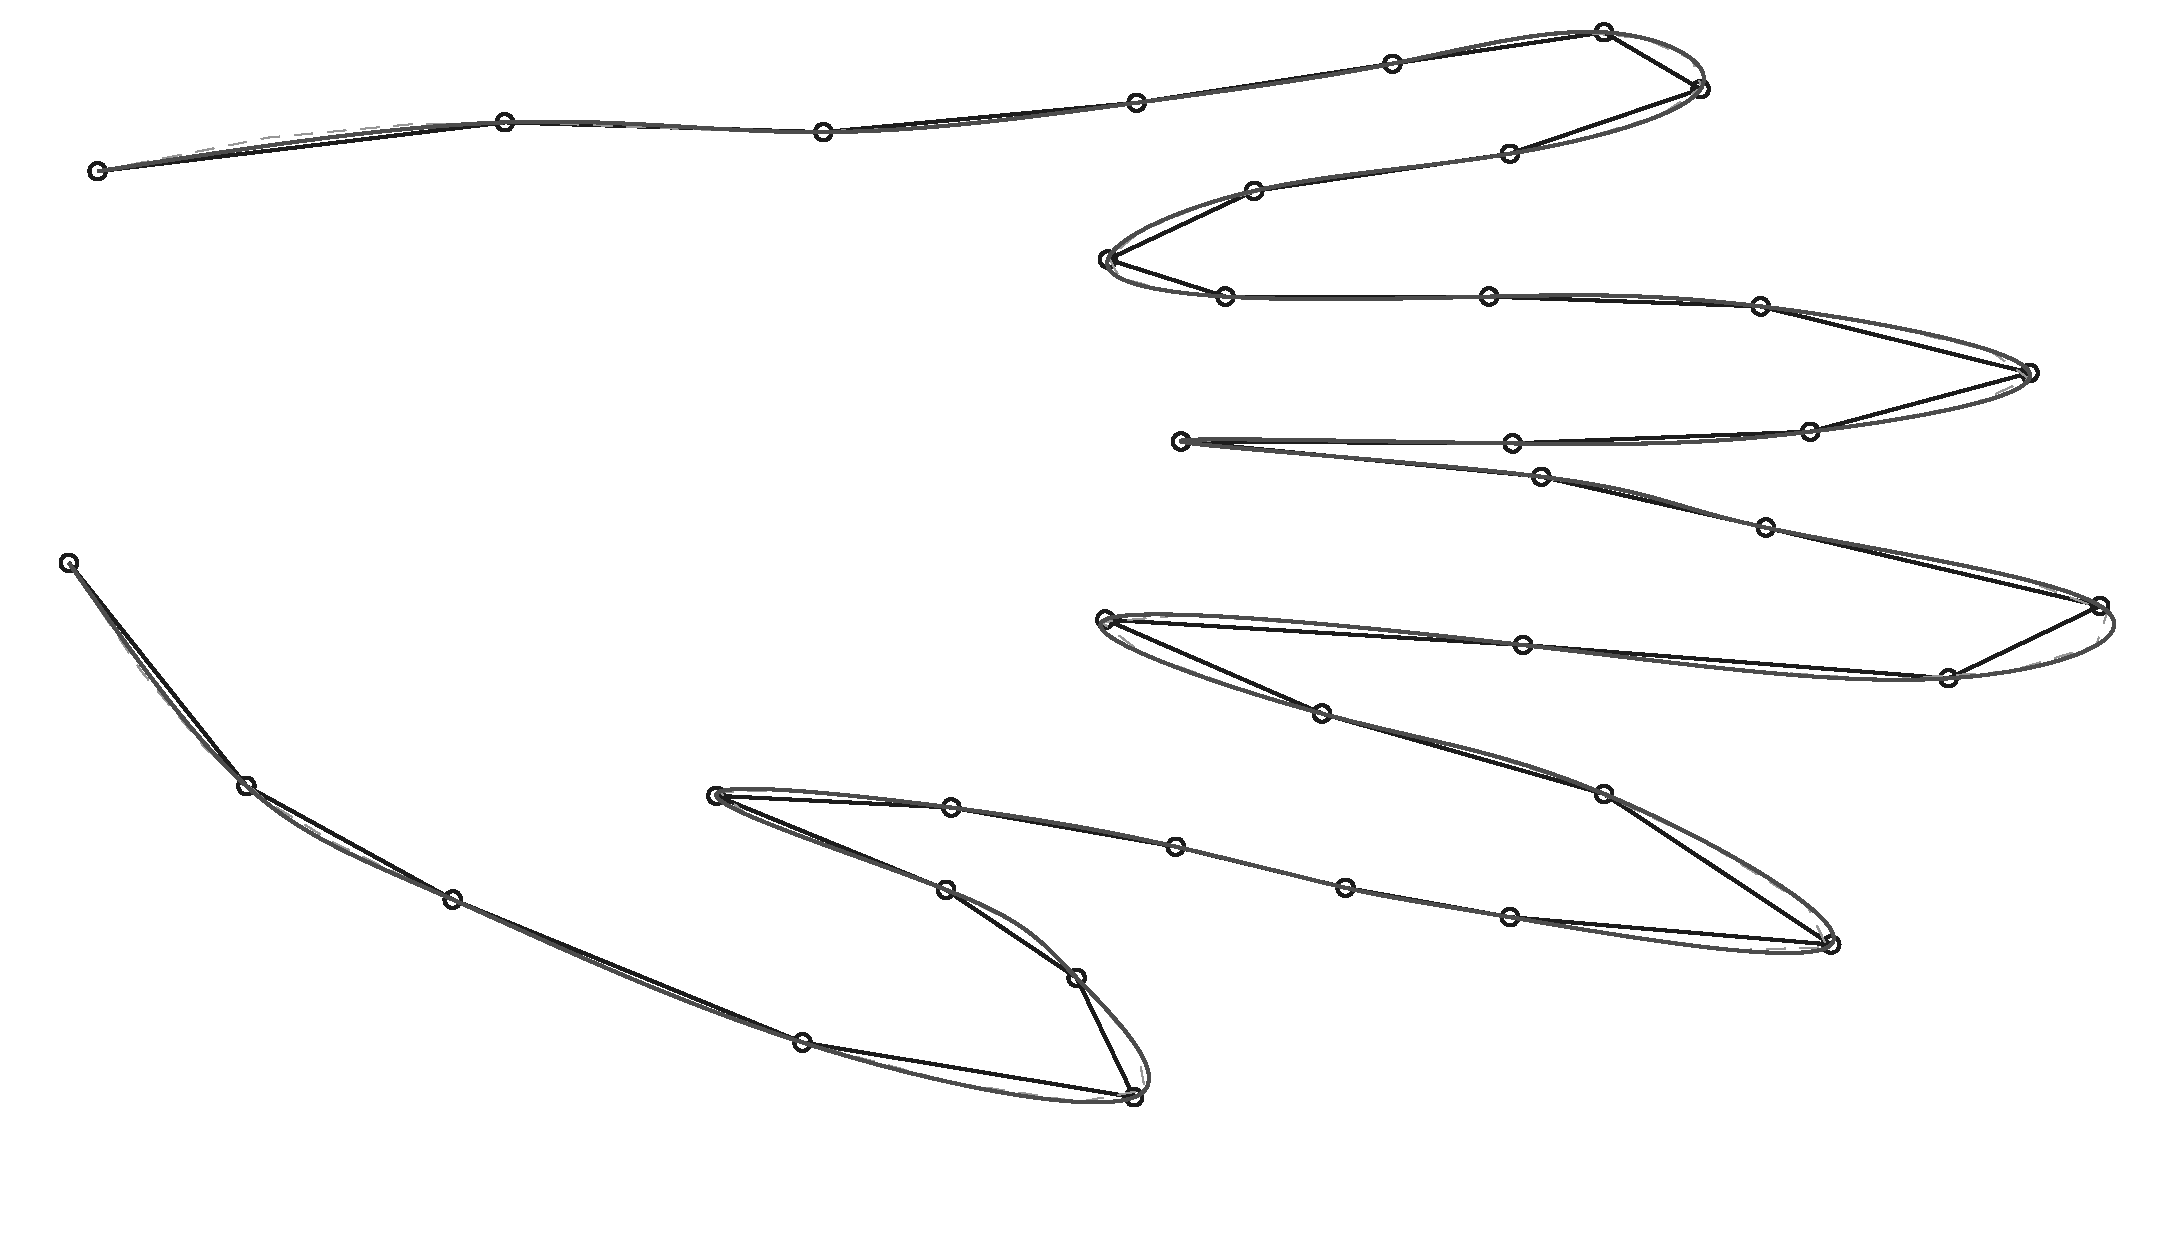
\includegraphics[scale=0.25]{Graficas/Mano1.eps}
\end{center}
El área aproximada fue 0.2479, como se observa la precisión es mejorable por lo que de ahora en adelante usaremos más puntos, observe con la misma mano la diferencia al escoger más puntos

\begin{center}
    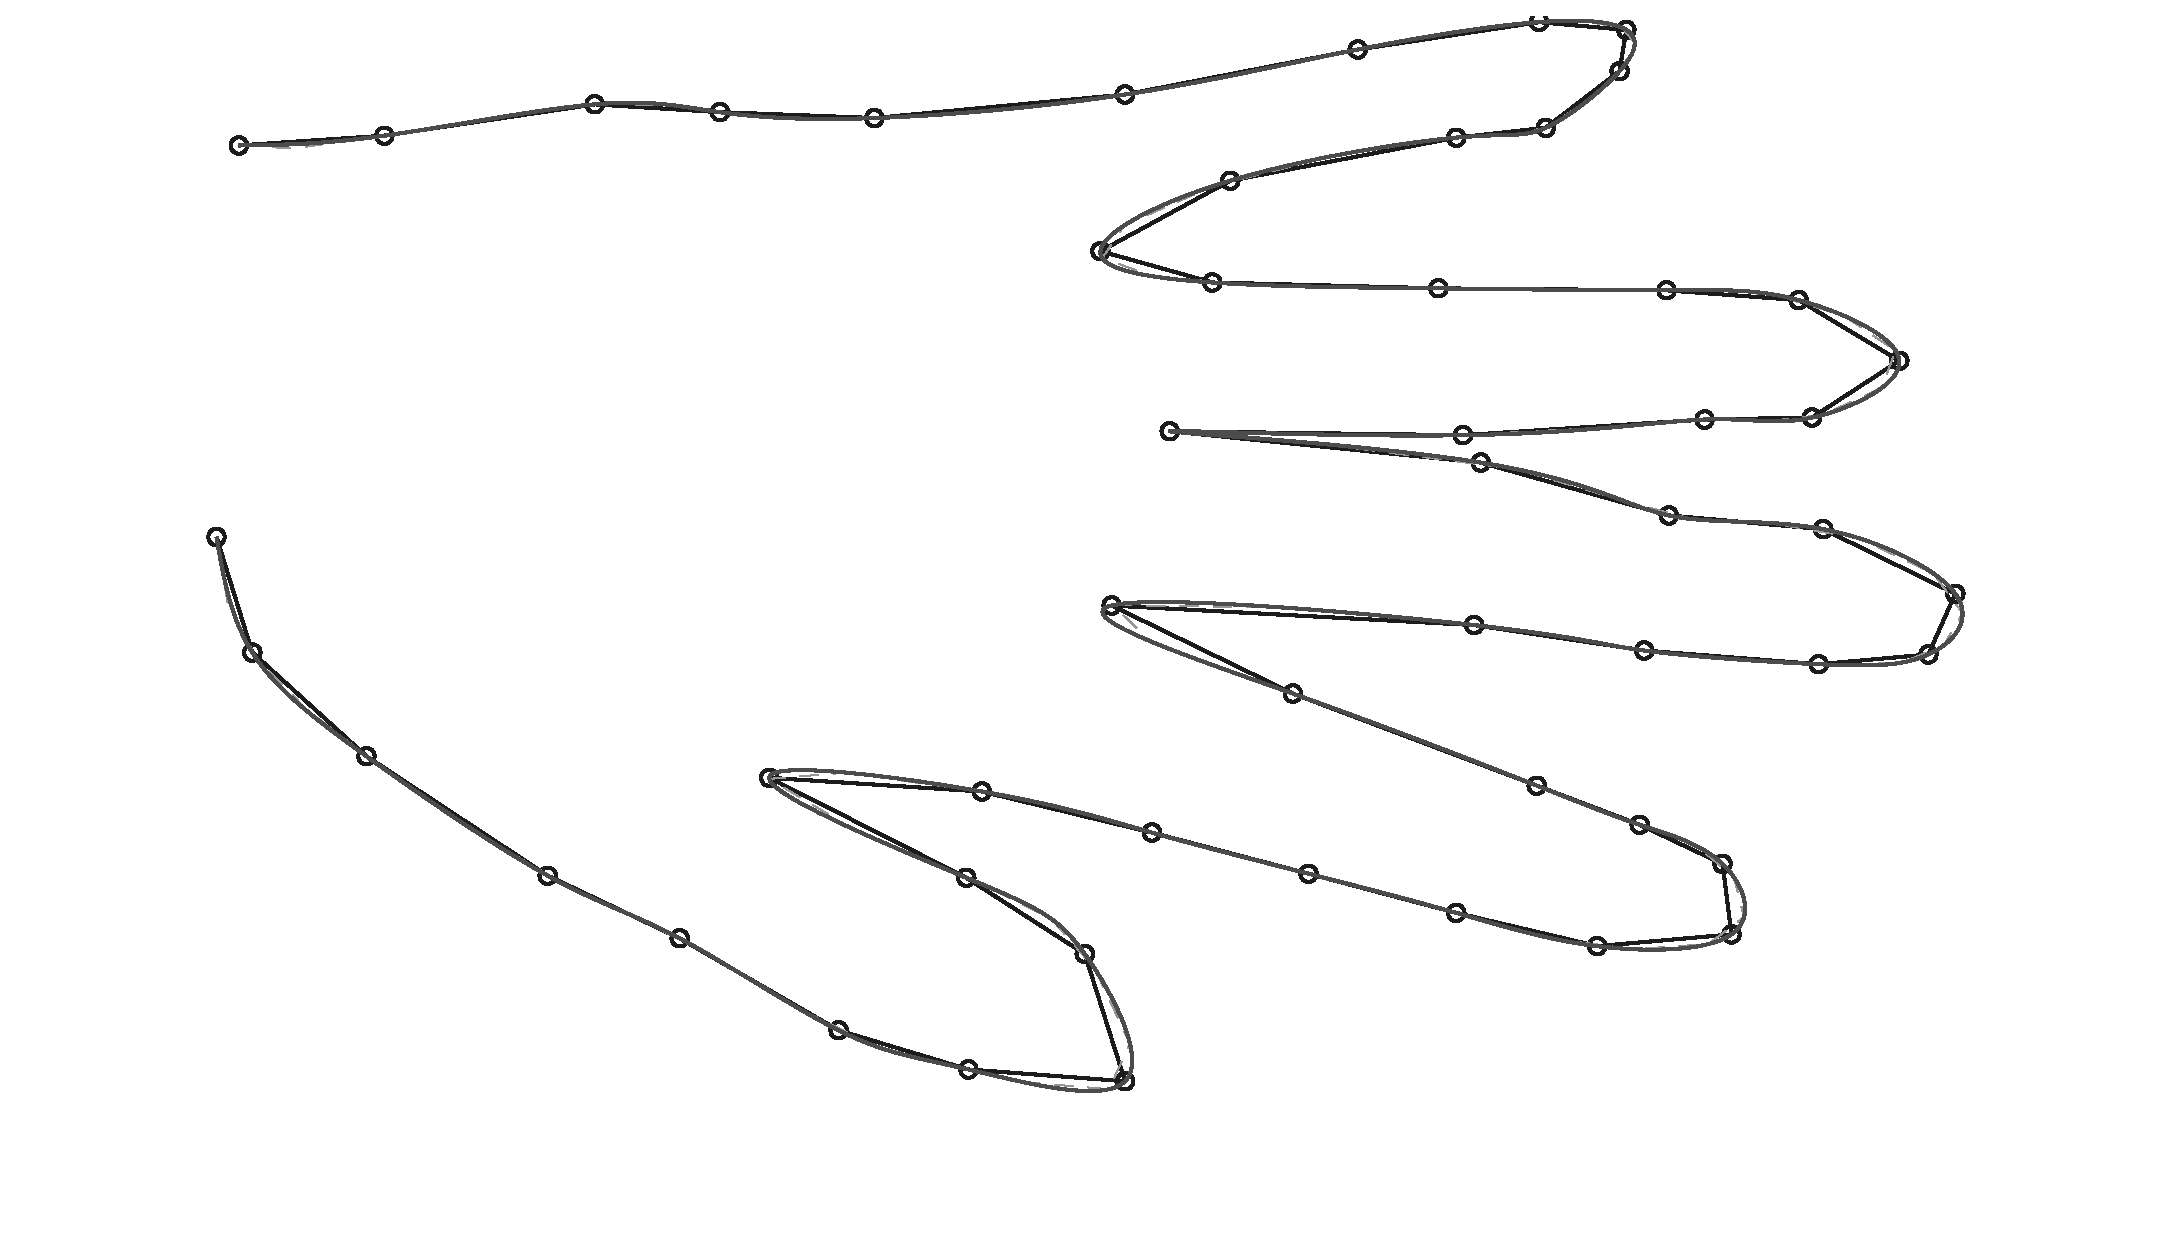
\includegraphics[scale=0.25]{Graficas/Mano1++.eps}
\end{center}

y obtenemos un área aproximada de 0.2533, es de esperar que en los parte donde los dedos se curvan se necesiten de más puntos. Para la segunda mano obtuvimos

\begin{center}
    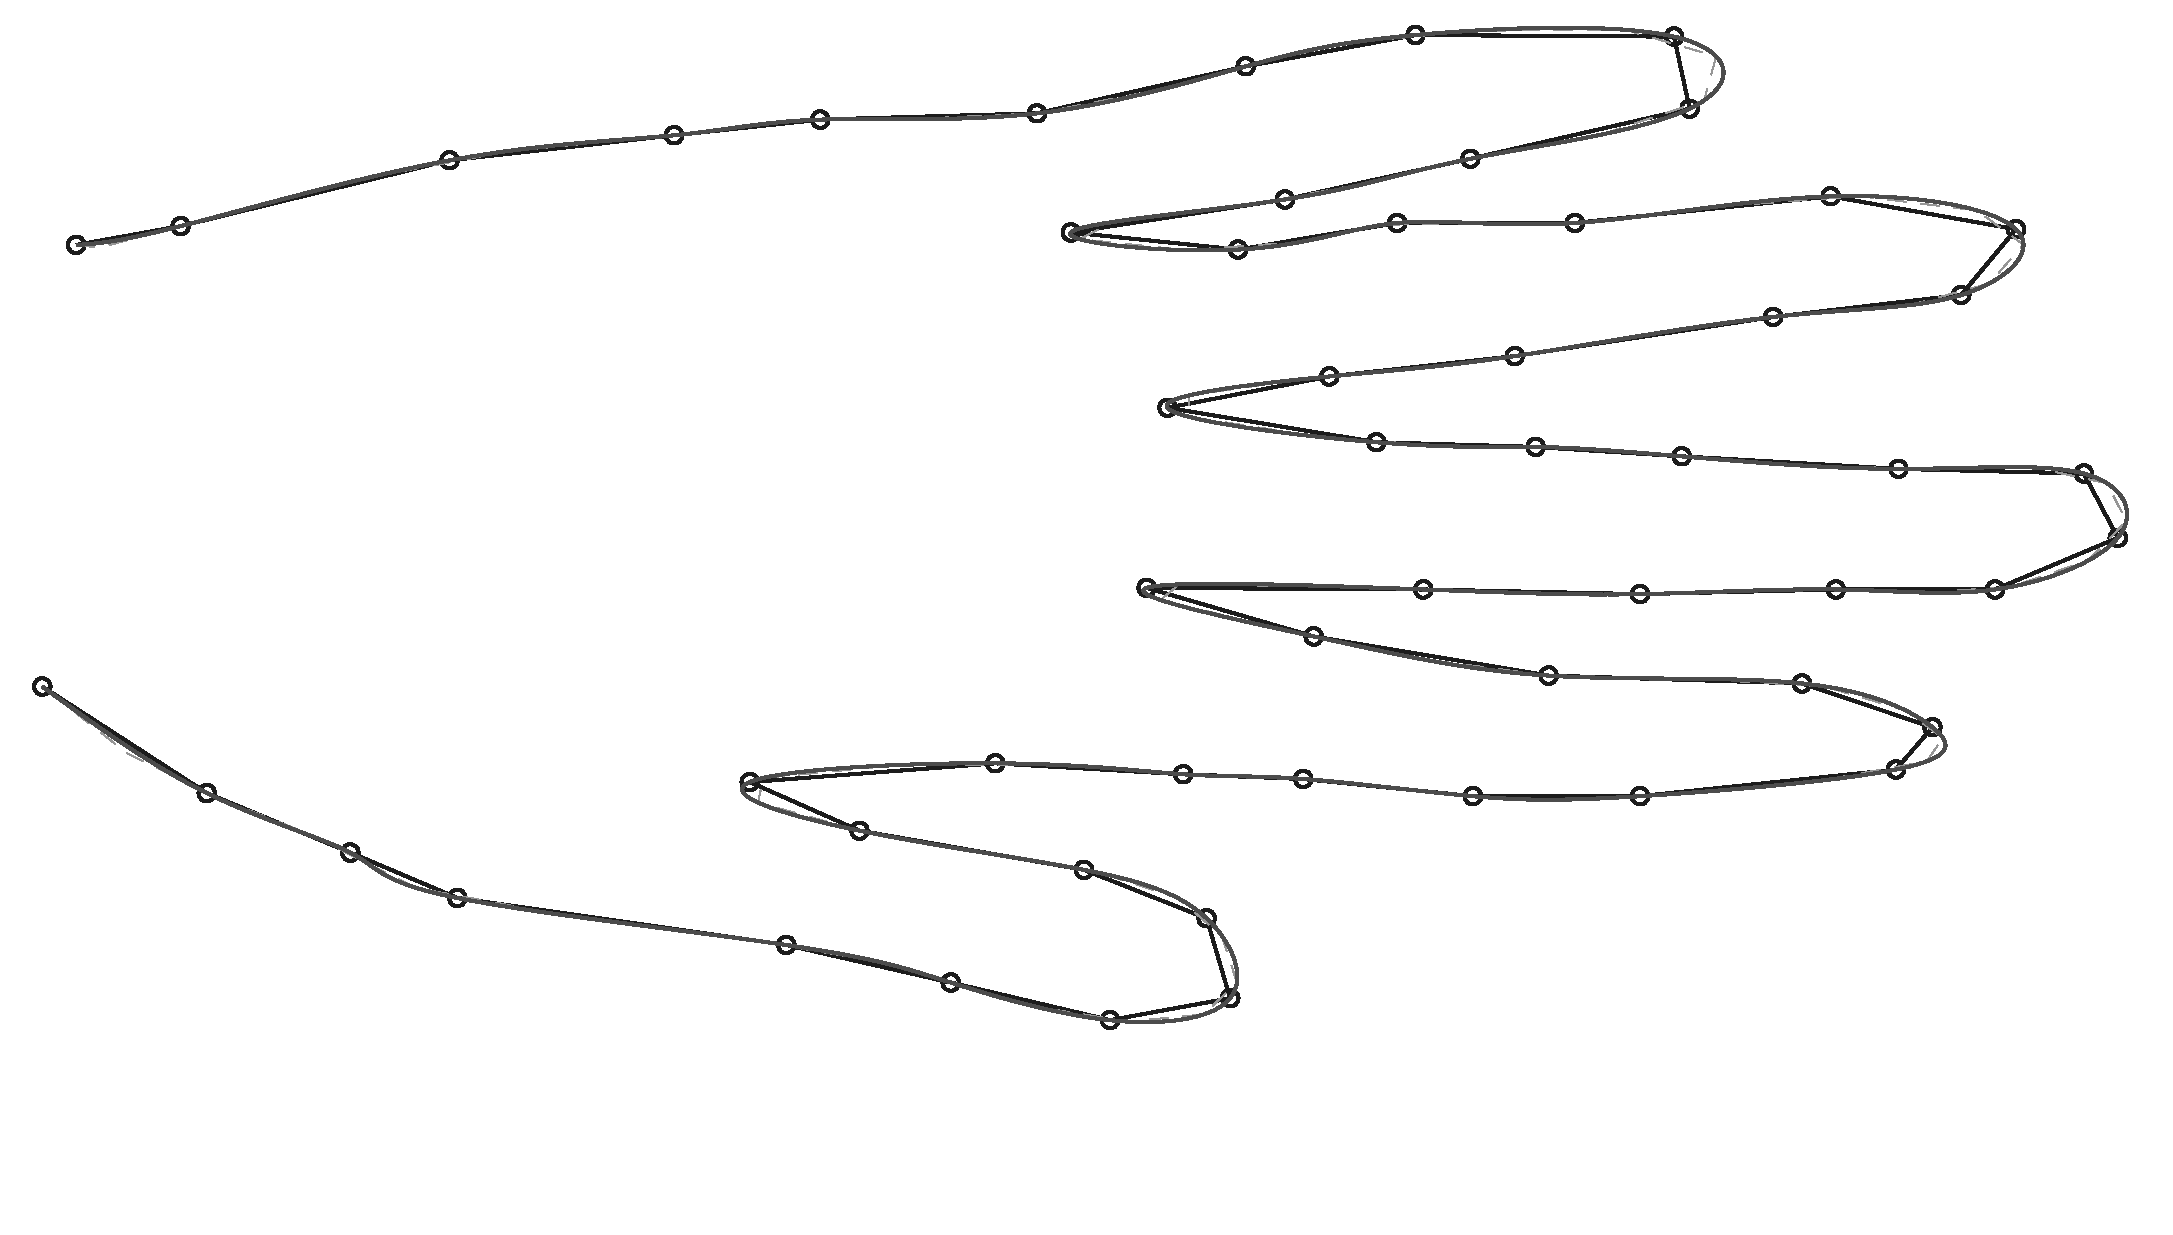
\includegraphics[scale=0.25]{Graficas/Mano2.eps}
\end{center}

y un área de 0.3121. \textcolor{red}{Alguno de ustedes hágalo con su mano porfa.}\\
\end{solution}

